\chapter{Target System and Threat Model}
\label{ch:target_system_threat_model}

This chapter formalises the adaptive learning pipeline targeted in this research and defines the capabilities and knowledge of an adversary attempting to compromise it. First, the architecture of the target system is detailed, consisting of a base learner coupled and an adversarially robust drift detector. Subsequently, a complete threat model is established, specifying the attacker's objectives, assumed knowledge, and operational capabilities.

\section{Target System Architecture}
The system under evaluation addresses concept drift in the typical way: by augmenting the base learner with a drift detector, as mentioned in \cref{sec:drift_detection}. However, this approach differs in that the supervisory module is dynamic. While traditional detectors rely on fixed statistical thresholds or heuristics, this architecture utilises a trainable drift detector. It learns a compressed latent representation of the known data distribution and measures deviation using class prototypes in that space to identify distributional shifts. This approach is intended to provide robustness to adversarial manipulation, a property which is scrutinised in the following chapters of this thesis.

The two components of the system, and the manner in which they are integrated, is described below.

\subsection{The Base Learner}
The base learner $\mathcal{M}$ is a binary multi-layer perceptron trained to classify the network flows as either \textsc{Benign} (class 0) or \textsc{Attack} (class 1). It consists of three fully-connected hidden layers of width 256, 128, 64 respectively, followed by a two-class output layer, giving:
\[
  \mathcal{M}: \mathbb{R}^{d} \;\to\; \mathbb{R}^{2}
\]

\subsection{The Drift Detector}
The drift detector $\mathcal{D}$ is the Contrastive Nearest Class Mean Detector (ContrastiveNCM)~\cite{Kuppa_2022}. Its architecture and training procedure are described in full in \cref{sec:contrastive_ncm}; here we only discuss the configuration choices specific to this experimental setup.

The encoder is trained with a latent dimension of $r = 32$, a hidden layer of width 64, and a contrastive temperature of $\tau = 0.1$, matching the hyperparameters reported in the original paper. The concept-discovery threshold is set to $T = 3.5$, again following the paper\cite{Kuppa_2022}.

\subsubsection{Drift threshold calibration}
The distance threshold $\tau_{\text{drift}}$, which determines whether an individual sample is flagged as drifted, is not fixed a priori. After initial training on the known-class data, it is set to the 95th percentile of NCM distances computed on a held-out calibration split containing only known-class instances. This yields a nominal false-positive rate of approximately 5\% on in-distribution traffic while correctly flagging novel-class samples, which are far from all known prototypes in the latent space. Crucially, the calibration requires no labels from novel classes, which is consistent with the deployment constraint that novel attacks have not yet been observed at training time.

\subsection{System Integration and Adaptation Cycle}
...
\todo[color=yellow]{Detail the exact adaptation mechanism here: e.g., Does it buffer new data to train a replacement tree in the background? Does it immediately discard the old tree?}

\begin{figure}[h]
    \centering
    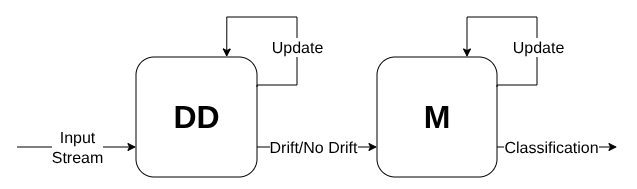
\includegraphics[width=\linewidth]{target_system_threat_model/target architecture.drawio.png}
    \caption{The general architecture of the target system}
    \label{fig:target architecture}
\end{figure}
\todo[color=yellow]{Figure can be improved}

\section{Threat Model}
To systematically evaluate the security of the target system, it is necessary to define the parameters under which an adversary operates. The threat model establishes the attacker's objectives, their level of knowledge about the system, and their practical capabilities within the environment.

\subsection{Attacker Objectives}
The primary objective of an adversary is to compromise the predictive accuracy or operational efficiency of the system as a whole. In this context, this manifests in two distinct ways:
\begin{itemize}
    \item \textit{Forcing False Adaptation}: The attacker aims to deceive the RRBM-DD into signalling a drift when the underlying distribution is stable, causing the Decision Tree to unnecessarily adapt to potentially malicious data, degrading its accuracy or consuming computational resources.

    \item \textit{Impairing Adaptation}: The attacker injects data that masks genuine concept drift in some way, preventing the RRBM-DD from detecting valid shifts and forcing the Decision Tree to rely on an outdated model.
\end{itemize}

\subsection{Attacker Knowledge}
The viability of an attack heavily depends on the adversary's understanding of the target system. The attacker's knowledge can be framed under 3 different assumptions:
\begin{itemize}
    \item \textit{White-Box:} The adversary possesses complete knowledge of the system. This includes but is not limited to the RRBM-DD's exact architecture, its current weights, the size of the mini-batches, and the specific statistical thresholds used in the Granger causality test.
   
    \item \textit{Grey-Box:} The adversary knows the general system architecture (e.g. that an RRBM-DD and a Decision Tree are being used) and the features of the data stream, but lacks access to the internal weights, sliding window states, or exact hyperparameters in real-time.
    
    \item \textit{Black-Box:} The adversary is unaware of the specific detection algorithms or base learner implemented. They can only observe the output predictions and the raw incoming data stream, meaning they must infer further details like the occurrence of a drift signal, based on changes in the system's external behaviour.
\end{itemize}

\subsection{Attacker Capabilities}
In the context of data stream mining, the adversary is assumed to have write access to the data ingestion pipeline, allowing them to manipulate the stream before it enters the predictive system. The adversary's capabilities are defined by the following constraints:
\begin{itemize}
    \item \textit{Feature Manipulation}: The ability to perturb the feature vector $X$ of incoming data points.
    
    \item \textit{Label Flipping}: The ability to alter the ground-truth label $y$ provided to the system.
    
    \item \textit{Injection Budget}: An adversary cannot replace 100\% of the stream, as this would trivially overwrite the system and would likely be flagged by upstream anomaly detection.
\end{itemize}